\documentclass[11pt]{article}

\usepackage{amsmath}
\usepackage{bm}
\usepackage{booktabs}
\usepackage{enumitem}
\usepackage[T1]{fontenc}
\usepackage[margin=1in]{geometry}
\usepackage[utf8]{inputenc}
\usepackage{libertine}
\usepackage[libertine]{newtxmath}
\usepackage{pgfplots}
\usepackage[detect-weight=true]{siunitx}

\title{MATH 128 End-of-Term Assignment 1}
\author{Brandon Tsang}
\date{March 29, 2020}

\pgfplotsset{compat=1.16}
\usetikzlibrary{arrows.meta}
\setlength{\parindent}{0pt}

\begin{document}
    \maketitle
    \begin{enumerate}[label={\textbf{\arabic*.}}]
        \item{
            \textbf{\boldmath Write out your student number and then determine the solution to each of the following initial value problems where $N_7$ and $N_8$ are the seventh and eighth digits of your student number:}
            \par
            My student number is 20845794.
            \begin{enumerate}[label={\textbf{(\alph*)}}]
                \item{
                    \textbf{\boldmath $\frac{dy}{dx}=y\cos(x),\quad y(0)=e^{N_7}$}
                    \par
                    This is a seperable differential equation. I'll solve it by separating the $y$'s from the $x$'s and integrating:
                    \begin{align*}
                        \frac{dy}{dx}&=y\cos(x) \\
                        \frac{1}{y}\,dy&=\cos(x)\,dx \\
                        \int\frac{1}{y}\,dy&=\int\cos(x)\,dx \\
                        \ln|y|&=\sin(x)+C \\
                        |y|&=e^{\sin(x)+C} \\
                        y&=\pm e^{\sin(x)}e^C
                    \end{align*}
                    Then, substituting $A=\pm e^C$:
                    \begin{equation}
                        y=Ae^{\sin(x)} \label{eqn:1a}
                    \end{equation}
                    The seventh digit of my student number is $N_7=9$, so
                    \begin{align*}
                        y(0)=e^{N_7}&=Ae^{\sin(0)} \\
                        e^9&=Ae^0 \\
                        A&=e^9.
                    \end{align*}
                    Substituting this back into equation \ref{eqn:1a}:
                    \begin{align*}
                        y&=e^9e^{\sin(x)} \\
                        &=e^{\sin(x)+9}
                    \end{align*}
                }
                \pagebreak
                \item{
                    \textbf{\boldmath $\frac{dy}{dx}+\frac{2}{x}y=x^{N_8},\quad y(1)=0$}
                    \par
                    This is a first-order linear differential equation in the form $y'+P(x)y=Q(x)$. First, I will rewrite the equation and find $P(x)$:
                    \begin{align}
                        \frac{dy}{dx}+\frac{2}{x}y&=x^{N_8} \nonumber \\
                        y'+\frac{2}{x}y&=x^{N_8} \label{eqn:1b1} \\
                        P(x)&=\frac{2}{x} \nonumber
                    \end{align}
                    Then, the integrating factor is $I(x)=e^{\int P(x)\,dx}$:
                    \begin{align*}
                        I(x)&=e^{\int P(x)\,dx} \\
                        &=e^{\int\frac{2}{x}\,dx} \\
                        &=e^{2\ln|x|} \\
                        &=e^{\ln(x^2)} \\
                        &=x^2
                    \end{align*}
                    Multiplying both sides of equation \ref{eqn:1b1} by $I(x)$:
                    \begin{align*}
                        x^2y'+x^2\frac{2}{x}y&=x^2x^{N_8} \\
                        \frac{d}{dx}(x^2y)&=x^{2+N_8}
                    \end{align*}
                    The eighth digit of my student number is $N_8=4$:
                    \begin{align}
                        \frac{d}{dx}(x^2y)&=x^{2+4} \nonumber \\
                        &=x^6 \nonumber \\
                        \int\frac{d}{dx}(x^2y)\,dx&=\int x^{6}\,dx \nonumber \\
                        x^2y&=\frac{x^7}{7}+C \nonumber \\
                        y&=\frac{x^5}{7}+C \label{eqn:1b2}
                    \end{align}
                    Next, I'm going to find $C$.
                    \begin{align*}
                        y(1)=0&=\frac{1^5}{7}+C \\
                        C&=-\frac{1}{7}
                    \end{align*}
                    Substituting $C$ back into equation \ref{eqn:1b2}:
                    \begin{align*}
                        y&=\frac{x^5}{7}+\left(-\frac{1}{7}\right) \\
                        &=\frac{x^5-1}{7}
                    \end{align*}
                }
            \end{enumerate}
        }
        \item{
            \textbf{
                \boldmath A patient receives periodic intravenous injections of a drug. Let $y(t)$ denote the drug concentration (in \si{\milli\gram\per\milli\liter}) in the patient's bloodstream at time $t$ with initial concentration $y(0)=L$.
                \begin{itemize}
                    \item Every $T$ time units, an injection increases the concentration by a quantity \SI[parse-numbers=false, number-math-rm=\mathnormal]{d}{\milli\gram\per\milli\liter}---that is, $y(t)$ increases by $d$ (a jump discontinuity) at times $t=T,2T,3T,$ \ldots.
                    \item In between doses, the drug concentration decreases exponentially, according to the differential equation $y'(t)=-ky(t)$ for some positive constant $k$.
                \end{itemize}
                Determine $T$ (as a function of $k$, $d$, and $L$) so that immediately after each dose, the value of $y(t)$ is $L$---that is, immediately before the dose, the value is $L-d$. (This is the most frequent dosing strategy that ensures the concentration is never above $L$.)
            }
            \par
            First, I'll solve the differential equation which is separable:
            \begin{align*}
                y'(t)&=-ky(t) \\
                \frac{dy}{dt}&=-ky \\
                \frac{1}{y}\,dy&=-k\,dt \\
                \int\frac{1}{y}\,dy&=\int-k\,dt \\
                \ln|y|&=-kt+C \\
                |y|&=e^{-kt+C} \\
                y&=\pm e^{-kt}e^C
            \end{align*}
            Substituting $A=\pm e^C$:
            \begin{equation}
                y=Ae^{-kt} \label{eqn:21}
            \end{equation}
            Then, to find $A$, I'll use the fact that $y(0)=L$.
            \begin{align*}
                y(0)=L&=Ae^{-k\cdot0} \\
                A&=L
            \end{align*}
            Substituting $A$ back into equation \ref{eqn:21}:
            $$y=Le^{-kt}$$
            Now, I'll find the time $t$ at which $y=L-d$:
            \begin{align*}
                L-d&=Le^{-kt} \\
                1-\frac{d}{L}&=e^{-kt} \\
                -kt&=\ln\left(1-\frac{d}{L}\right) \\
                t&=-\frac{1}{k}\ln\left(1-\frac{d}{L}\right)
            \end{align*}
            This is the amount of time after $t=0$ at which the first injection is needed. Since the concentration of the drug decreases by the same curve each time, $T=t=-\frac{1}{k}\ln\left(1-\frac{d}{L}\right)$.
        }
        \item{
            \textbf{\boldmath Glaciers are rivers of ice. The point at which a glacier ends is called its \textit{terminus}. The thickness, $T$, of a glacier can be described as a function of the distance $x$ from the terminus: $T=T(x)$. That thickness function can be shown to satisfy the differential equation $$T\frac{dT}{dx}=\frac{\tau}{\rho g}$$ where $\tau$ is the coefficient of friction at the bottom of the glacier, $\rho$ is the density of ice in the glacier, and $g$ is acceleration due to gravity.}
            \begin{enumerate}[label={\textbf{(\alph*)}}]
                \item{
                    \textbf{What is the order of this differential equation?}
                    \par
                    The order is 1.
                }
                \item{
                    \textbf{Is this differential equation separable? Is it linear?}
                    \par
                    It is separable (in fact, it's already separated), but it is not linear as $T$ is in the same term as its derivative.
                }
                \item{
                    \textbf{Determine the general solution of the differential equation model.}
                    \par
                    The differential equation is solved as follows:
                    \begin{align*}
                        T\frac{dT}{dx}&=\frac{\tau}{\rho g} \\
                        T\,dT&=\frac{\tau}{\rho g}\,dx \\
                        \int T\,dT&=\int\frac{\tau}{\rho g}\,dx \\
                        \frac{1}{2}T^2&=\frac{\tau}{\rho g}x+C \\
                        T^2&=\frac{2\tau}{\rho g}x+C \\
                        T&=\sqrt{\frac{2\tau}{\rho g}x+C}
                    \end{align*}
                }
                \item{
                    \textbf{\raggedright\boldmath Given the initial condition $T(0)=0$, determine the thickness of the glacier at a distance of \SI{1}{\kilo\meter} from its terminus. Take $\rho=\SI{917}{\kilogram\per\cubic\meter}$, $g=\SI{9.8}{\meter\per\square\second}$, and\\$\tau=\SI{75000}{\newton\per\square\meter}$.}
                    \par
                    First, I'll find the value of $C$ using the inital value $T(0)=0$:
                    \begin{align*}
                        T(0)=0&=\sqrt{\frac{2\tau}{\rho g}\cdot0+C} \\
                        C&=0
                    \end{align*}
                    Therefore, $T=\sqrt{\frac{2\tau}{\rho g}x}$.
                    \begin{align*}
                        T(\SI{1000}{\meter})&=\sqrt{\frac{2\tau}{\rho g}x} \\
                        &=\sqrt{\frac{2(\SI{75000}{\newton\per\square\meter})}{(\SI{917}{\kilogram\per\cubic\meter})(\SI{9.8}{\meter\per\square\second})}\cdot\SI{1000}{\meter}} \\
                        &=\SI{129.196}{\meter}
                    \end{align*}
                }
            \end{enumerate}
        }
        \item{
            \textbf{\boldmath Consider the initial value problem $$\frac{dy}{dt}=y+t,\quad y(0)=1$$}
            \begin{enumerate}[label={\textbf{(\alph*)}}]
                \item{
                    \textbf{\boldmath Construct a direction (slope) field for the differential equation on a plot with\\$-2\le t\le2$ and $0\le y\le4$ showing slopes at all 25 lattice points. On your direction (slope) field, sketch the solution curve which satisfies the given initial value problem.}
                    \begin{center}
                        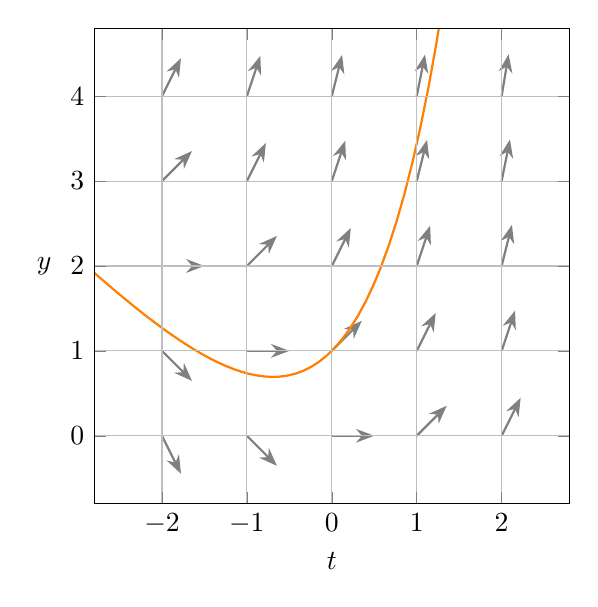
\begin{tikzpicture}
                            \def\length{sqrt(1+(y+x)^2)}
                            \begin{axis}[
                                width=3in,
                                height=3in,
                                xmin=-2, xmax=2,
                                ymin=0, ymax=4,
                                zmin=-1, zmax=1,
                                enlargelimits=0.2,
                                xlabel={$t$},
                                ylabel={$y$},
                                ylabel style={rotate=-90},
                                grid=major,
                                xtick distance=1,
                                ytick distance=1,
                                view={0}{90}
                            ]
                                \addplot3[
                                    -Stealth,
                                    thick,
                                    gray,
                                    domain=-2:2,
                                    y domain=0:4,
                                    samples=5,
                                    quiver={
                                        u={1/(\length)},
                                        v={(y+x)/(\length)},
                                        scale arrows=0.5,
                                    }
                                ] {0};
                                \addplot[mark=none, orange, thick, domain=-3:1.5, samples=50] {-x-1+2*e^x};
                            \end{axis}
                        \end{tikzpicture}
                    \end{center}
                }
                \item{
                    \textbf{\boldmath Determine the exact solution to this initial value problem and report the value of $y(0.2)$.}
                    \par
                    The differential equation is first-order and linear. I'll start by rewriting the equation into the form $y'+P(t)y=Q(t)$:
                    \begin{align}
                        \frac{dy}{dt}&=y+t \nonumber \\
                        y'-y&=t \label{eqn:4b1}
                    \end{align}
                    The integrating factor is $I(t)=e^{\int P(t)\,dt}$:
                    \begin{align*}
                        I(t)&=e^{\int-1\,dt} \\
                        &=e^{-t}
                    \end{align*}
                    Multiplying both sides of equation \ref{eqn:4b1} by $I(t)$:
                    \begin{align}
                        e^{-t}y'-e^{-t}y&=e^{-t}t \nonumber \\
                        \frac{d}{dt}(e^{-t}y)&=e^{-t}t \nonumber \\
                        \int\frac{d}{dt}(e^{-t}y)\,dt&=\int e^{-t}t\,dt \nonumber \\
                        e^{-t}y&=\int e^{-t}t\,dt & \begin{aligned}u&=t & v&=-e^{-t} \\ du&=dt & dv&=e^{-t}\,dt\end{aligned} \nonumber \\
                        &=-te^{-t}-\int-e^{-t}\,dt \nonumber \\
                        &=-te^{-t}-e^{-t}+C \nonumber \\
                        y&=Ce^t-t-1 \label{eqn:4b2}
                    \end{align}
                    To find $C$, I'll use the initial value $y(0)=1$.
                    \begin{align*}
                        y(0)=1&=Ce^0-0-1 \\
                        &=C-1 \\
                        C&=2
                    \end{align*}
                    Plugging $C$ back into equation \ref{eqn:4b2}:
                    $$y=2e^t-t-1$$
                    Now, I can find $y(0.2)$:
                    \begin{align*}
                        y(0.2)&=2e^{0.2}-0.2-1 \\
                        &=1.24280\ldots
                    \end{align*}
                }
            \end{enumerate}
            \textbf{\boldmath Recall, Euler's method can be used to approximate the solution to the initial value problem $$y'(t)=f(t,y(t)),\quad y(0)=y_0$$ by applyng the update rule $$y(t+h)=y(t)+hf(t,y(t))$$}
            \begin{enumerate}[label={\textbf{(\alph*)}}, resume]
                \item{
                    \textbf{\boldmath Take $h=0.1$ and use Euler's method to approximate the value of $y(0.2)$.}
                    \par
                    Starting with $t=0$ and $y(0)=1$:
                    \begin{align*}
                        y(0+0.1)&=1+0.1(1+0) \\
                        y(0.1)&=1.1 \\[8pt]
                        y(0.1+0.1)&=1.1+0.1(1.1+0.1) \\
                        y(0.2)&=1.22
                    \end{align*}
                }
            \end{enumerate}
            \textbf{\boldmath More accuracy can be achieved by applying Euler's midpoint method, which has the update rule $$y(t+h)=y(t)+hm(t,y(t))$$ where the function $m$ is defined by $$m(t,y(t))=f\left(t+\frac{h}{2},y(t)+\frac{h}{2}f(t,y(t))\right)$$}
            \begin{enumerate}[label={\textbf{(\alph*)}}, resume]
                \item{
                    \textbf{\boldmath Take $h=0.1$ and use Euler's midpoint method to approximate the value of $y(0.2)$.}
                    \par
                    Starting with $t=0$ and $y(0)=1$:
                    \begin{align*}
                        y(0+0.1)&=1+0.1\left(0+\frac{0.1}{2}+1+\frac{0.1}{2}(1+0)\right) \\
                        y(0.1)&=1.11 \\[8pt]
                        y(0.1+0.1)&=1.11+0.1\left(0.1+\frac{0.1}{2}+1.11+\frac{0.1}{2}(1.11+0.1)\right) \\
                        y(0.2)&=1.24205
                    \end{align*}
                }
            \end{enumerate}
        }
        \pagebreak
        \item{
            \textbf{\boldmath Our goal in this question is to model the behaviour of a mass on a spring with and without friction. In both cases, we'll seek the solution to a differential equation of the form: \begin{equation}a\frac{d^2x}{dt^2}+b\frac{dx}{dt}+cx=0\label{eqn:5}\end{equation} where $x=x(t)$ is a function of time $t$ and $a$, $b$, and $c$ are constant real numbers.}
            \begin{enumerate}[label={\textbf{(\alph*)}}]
                \item{
                    \label{part:5a}
                    \textbf{\boldmath Show that the differential equation is satisfied by $x(t)=e^{rt}(C_1\cos(\omega t)+C_2\sin(\omega t))$ where $r=-\frac{b}{2a}$ and $\omega=\frac{\sqrt{4ac-b^2}}{2a}$. (Note, this equation for $x(t)$ is the \textit{general solution} to the DE when $b^2-4ac<0$ so that $\omega$ is a non-zero real number.)}
                    \par
                    First, I'll find the first and second derivatives of $x(t)$:
                    \begin{align*}
                        x(t)=x&=e^{rt}(C_1\cos(\omega t)+C_2\sin(\omega t)) \\[8pt]
                        \frac{dx}{dt}&=re^{rt}(C_1\cos(\omega t)+C_2\sin(\omega t))+e^{rt}(-\omega C_1\sin(\omega t)+\omega C_2\cos(\omega t)) \\
                        &=e^{rt}(rC_1\cos(\omega t)+rC_2\sin(\omega t)-\omega C_1\sin(\omega t)+\omega C_2\cos(\omega t))
                    \end{align*}
                    This is getting a little unwieldly. I'm going to define a new function $w(t)=rC_1\cos(\omega t)+rC_2\sin(\omega t)-\omega C_1\sin(\omega t)+\omega C_2\cos(\omega t)$ to break it up a little. Now, the first derivative looks like
                    $$\frac{dx}{dt}=e^{rt}w(t)$$
                    which is much nicer.
                    \par
                    Let's find the second derivative.
                    \begin{align*}
                        \frac{d^2x}{dt^2}&=re^{rt}w(t)+e^{rt}w'(t)
                    \end{align*}
                    Finding $w'(t)$:
                    \begin{align*}
                        w'(t)&=-r\omega C_1\sin(\omega t)+r\omega C_2\cos(\omega t)-\omega^2C_1\cos(\omega t)-\omega^2C_2\sin(\omega t)
                    \end{align*}
                    Before I start plugging the derivatives into equation \ref{eqn:5}, I'm going to expand out all the terms to make things neater. Starting with $x$:
                    \begin{align*}
                        x&=e^{rt}(C_1\cos(\omega t)+C_2\sin(\omega t)) \\
                        &=C_1e^{rt}\cos(\omega t)+C_2e^{rt}\sin(\omega t)
                    \end{align*}
                    Next, $\frac{dx}{dt}$:
                    \begin{align*}
                        \frac{dx}{dt}&=e^{rt}(rC_1\cos(\omega t)+rC_2\sin(\omega t)-\omega C_1\sin(\omega t)+\omega C_2\cos(\omega t)) \\
                        &=C_1re^{rt}\cos(\omega t)+C_2re^{rt}\sin(\omega t)-C_1\omega e^{rt}\sin(\omega t)+C_2\omega e^{rt}\cos(\omega t)
                    \end{align*}
                    And finally, $\frac{d^2x}{dt^2}$:
                    \begin{align*}
                        \begin{split}
                            \frac{d^2x}{dt^2}&=re^{rt}(rC_1\cos(\omega t)+rC_2\sin(\omega t)-\omega C_1\sin(\omega t)+\omega C_2\cos(\omega t)) \\
                            &\phantom{=}\quad {}+e^{rt}(-r\omega C_1\sin(\omega t)+r\omega C_2\cos(\omega t)-\omega^2C_1\cos(\omega t)-\omega^2C_2\sin(\omega t))
                        \end{split} \\[8pt]
                        \begin{split}
                            &=C_1r^2e^{rt}\cos(\omega t)+C_2r^2e^{rt}\sin(\omega t)-C_1r\omega e^{rt}\sin(\omega t)+C_2r\omega e^{rt}\cos(\omega t) \\
                            &\phantom{=}\quad {}-C_1r\omega e^{rt}\sin(\omega t)+C_2r\omega e^{rt}\cos(\omega t)-C_1\omega^2e^{rt}\cos(\omega t)-C_2\omega^2e^{rt}\sin(\omega t)
                        \end{split}
                    \end{align*}
                    Now I can finally start plugging into equation \ref{eqn:5}.
                    \begin{equation*}
                        \begin{split}
                            a(C_1r^2e^{rt}\cos(\omega t)+C_2r^2e^{rt}\sin(\omega t)-C_1r\omega e^{rt}\sin(\omega t)+C_2r\omega e^{rt}\cos(\omega t)\quad&\\
                            -C_1r\omega e^{rt}\sin(\omega t)+C_2r\omega e^{rt}\cos(\omega t)-C_1\omega^2e^{rt}\cos(\omega t)-C_2\omega^2e^{rt}\sin(\omega t))\quad&\\
                            +b(C_1re^{rt}\cos(\omega t)+C_2re^{rt}\sin(\omega t)-C_1\omega e^{rt}\sin(\omega t)+C_2\omega e^{rt}\cos(\omega t))\quad&\\
                            +c(C_1e^{rt}\cos(\omega t)+C_2e^{rt}\sin(\omega t))&=0
                        \end{split}
                    \end{equation*}
                    Expanding, I get:
                    \begin{equation*}
                        \begin{split}
                            C_1ar^2e^{rt}\cos(\omega t)+C_2ar^2e^{rt}\sin(\omega t)-C_1ar\omega e^{rt}\sin(\omega t)+C_2ar\omega e^{rt}\cos(\omega t)\quad&\\
                            -C_1ar\omega e^{rt}\sin(\omega t)+C_2ar\omega e^{rt}\cos(\omega t)-C_1a\omega^2e^{rt}\cos(\omega t)-C_2a\omega^2e^{rt}\sin(\omega t)\quad&\\
                            +C_1bre^{rt}\cos(\omega t)+C_2bre^{rt}\sin(\omega t)-C_1b\omega e^{rt}\sin(\omega t)+C_2b\omega e^{rt}\cos(\omega t)\quad&\\
                            +C_1ce^{rt}\cos(\omega t)+C_2ce^{rt}\sin(\omega t)&=0
                        \end{split}
                    \end{equation*}
                    Then, I'm going to group the terms by cosines and sines.
                    \begin{equation*}
                        \begin{alignedat}{7}
                            &(&C_1ar^2e^{rt}&\cos(\omega t)&{}+{}&C_2ar\omega e^{rt}&\cos(\omega t)&{}+{}&C_2ar\omega e^{rt}&\cos(\omega t)&{}-{}&C_1a\omega^2e^{rt}&\cos(\omega t) \\
                            {}+{}&&C_1bre^{rt}&\cos(\omega t)&{}+{}&C_2b\omega e^{rt}&\cos(\omega t)&{}+{}&C_1ce^{rt}&\cos(\omega t)) \\
                            {}+{}&(&C_2ar^2e^{rt}&\sin(\omega t)&{}-{}&C_1ar\omega e^{rt}&\sin(\omega t)&{}-{}&C_1ar\omega e^{rt}&\sin(\omega t)&{}-{}&C_2a\omega^2e^{rt}&\sin(\omega t) \\
                            {}+{}&&C_2bre^{rt}&\sin(\omega t)&{}-{}&C_1b\omega e^{rt}&\sin(\omega t)&{}+{}&C_2ce^{rt}&\sin(\omega t))&&&&=0
                        \end{alignedat}
                    \end{equation*}
                    Now, I can factor out the cosines and sines, as well as $e^{rt}$.
                    \begin{align*}
                        \begin{alignedat}{2}
                            &e^{rt}\cos(\omega t)(C_1ar^2+C_2ar\omega+C_2ar\omega-C_1a\omega^2+C_1br+C_2b\omega+C_1c)& \\
                            {}+{}&e^{rt}\sin(\omega t)(C_2ar^2+C_1ar\omega+C_1ar\omega-C_2a\omega^2+C_2br+C_1b\omega+C_2c)&{}=0
                        \end{alignedat} \\[8pt]
                        \begin{alignedat}{2}
                            &e^{rt}\cos(\omega t)(C_1ar^2+2C_2ar\omega-C_1a\omega^2+C_1br+C_2b\omega+C_1c)& \\
                            {}+{}&e^{rt}\sin(\omega t)(C_2ar^2+2C_1ar\omega-C_2a\omega^2+C_2br+C_1b\omega+C_2c)&{}=0
                        \end{alignedat}
                    \end{align*}
                    Let's put the expressions for $r$ and $\omega$ in.
                    \begin{align*}
                        \begin{split}
                            e^{rt}\cos(\omega t)\bigg(C_1a\left(-\tfrac{b}{2a}\right)^2+2C_2a\left(-\tfrac{b}{2a}\right)\left(\tfrac{\sqrt{4ac-b^2}}{2a}\right)\qquad&\\
                            {}-C_1a\left(\tfrac{\sqrt{4ac-b^2}}{2a}\right)^2+C_1b\left(-\tfrac{b}{2a}\right)+C_2b\left(\tfrac{\sqrt{4ac-b^2}}{2a}\right)+C_1c\bigg)\quad& \\
                            {}+e^{rt}\sin(\omega t)\bigg(C_2a\left(-\tfrac{b}{2a}\right)^2{}+2C_1a\left(-\tfrac{b}{2a}\right)\left(\tfrac{\sqrt{4ac-b^2}}{2a}\right)\qquad&\\
                            {}-C_2a\left(\tfrac{\sqrt{4ac-b^2}}{2a}\right)^2+C_2b\left(-\tfrac{b}{2a}\right)+C_1b\left(\tfrac{\sqrt{4ac-b^2}}{2a}\right)+C_2c\bigg)&=0
                        \end{split} \\[8pt]
                        \begin{split}
                            e^{rt}\cos(\omega t)\left(C_1\tfrac{b^2}{4a}-C_2\tfrac{b\sqrt{4ac-b^2}}{2a}-C_1\tfrac{4ac-b^2}{4a}-C_1\tfrac{b^2}{2a}+C_2\tfrac{b\sqrt{4ac-b^2}}{2a}+C_1c\right)\quad& \\
                            {}+e^{rt}\sin(\omega t)\left(C_2\tfrac{b^2}{4a}-C_1\tfrac{b\sqrt{4ac-b^2}}{2a}-C_2\tfrac{4ac-b^2}{4a}-C_2\tfrac{b^2}{2a}+C_1\tfrac{b\sqrt{4ac-b^2}}{2a}+C_2c\right)&=0
                        \end{split} \\
                        \begin{split}
                            e^{rt}\cos(\omega t)\left(C_1\tfrac{b^2}{4a}-C_1\tfrac{4ac-b^2}{4a}-C_1\tfrac{b^2}{2a}+C_1c\right)\quad& \\
                            {}+e^{rt}\sin(\omega t)\left(C_2\tfrac{b^2}{4a}-C_2\tfrac{4ac-b^2}{4a}-C_2\tfrac{b^2}{2a}+C_2c\right)&=0
                        \end{split}
                    \end{align*}
                    Now I can factor out $C_1$ and $C_2$.
                    \begin{align*}
                        C_1e^{rt}\cos(\omega t)\left(\tfrac{b^2}{4a}-\tfrac{4ac-b^2}{4a}-\tfrac{b^2}{2a}+c\right)+C_2e^{rt}\sin(\omega t)\left(\tfrac{b^2}{4a}-\tfrac{4ac-b^2}{4a}-\tfrac{b^2}{2a}+c\right)&=0 \\
                        \left(\frac{b^2}{4a}-\frac{4ac-b^2}{4a}-\frac{b^2}{2a}+c\right)(C_1e^{rt}\cos(\omega t)+C_2e^{rt}\sin(\omega t))&=0 \\
                        \left(\frac{b^2-4ac+b^2-2b^2+4ac}{4a}\right)(C_1e^{rt}\cos(\omega t)+C_2e^{rt}\sin(\omega t))&=0 \\
                        (0)(C_1e^{rt}\cos(\omega t)+C_2e^{rt}\sin(\omega t))&=0 \\
                        0&=0\qquad\raisebox{-4pt}{
\includegraphics{partypopper.png}}
                    \end{align*}
                }
            \end{enumerate}
            \textbf{\boldmath Now, consider a mass $m$ attached to a spring with spring constant $k$ (which quantifies the stiffness of the spring). The spring exerts a force on the mass proportional to the extension/compression of the spring from equilibrium. Let us denote the extension of the spring at a time $t$ by $x(t)$. Ignoring friction, Newton's second law gives the differential equation $$m\frac{d^2x}{dt^2}+kx=0$$}
            \begin{enumerate}[label={\textbf{(\alph*)}}, resume]
                \item{
                    \label{part:5b}
                    \textbf{Determine the general solution to this DE using information given in the part \ref{part:5a} of this question.}
                    \par
                    According to part \ref{part:5a}, the general solution to a second-order linear differential equation of the form $a\frac{d^2x}{dt^2}+b\frac{dx}{dt}+cx=0$ is given by $$x=e^{rt}(C_1\cos(\omega t)+C_2\sin(\omega t))$$ where $r=-\frac{b}{2a}$ and $\omega=\frac{\sqrt{4ac-b^2}}{2a}$.
                    \par
                    Plugging in $a=m$, $b=0$, and $c=k$, $r$ becomes 0 and $\omega$ becomes $\frac{\sqrt{4mk}}{2m}$. Putting $r=0$ and $\omega=\frac{\sqrt{4mk}}{2m}$ into the general solution, we get:
                    \begin{align*}
                        x&=e^{0t}\left(C_1\cos\left(\tfrac{\sqrt{4mk}}{2m}t\right)+C_2\sin\left(\tfrac{\sqrt{4mk}}{2m}t\right)\right) \\
                        &=C_1\cos\left(\tfrac{\sqrt{4mk}}{2m}t\right)+C_2\sin\left(\tfrac{\sqrt{4mk}}{2m}t\right)
                    \end{align*}
                }
                \item{
                    \label{part:5c}
                    \textbf{\boldmath Choose initial conditions (that do not give $x(t)=0$) and set $m=N_7+1$ and $k=N_8+1$ where $N_7$ and $N_8$ are the seventh and eighth digits of your student number. Sketch the corresponding solution for values of $t\ge0$.}
                    \par
                    Setting $m=N_7+1=10$ and $k=N_8+1=5$, the general solution becomes:
                    \begin{equation*}
                        x=C_1\cos\left(\frac{\sqrt{200}}{20}t\right)+C_2\sin\left(\frac{\sqrt{200}}{20}t\right)
                    \end{equation*}
                    Since there are two unknowns, I'll pick two constraints to find a solution. These will be $$\begin{matrix}t_1=0 & t_2=6 \\ x(t_1)=3 & x(t_2)=5\end{matrix}$$ Now I'll use them to find $C_1$ and $C_2$.
                    \begin{align*}
                        x(0)=3&=C_1\cos\left(\tfrac{\sqrt{200}}{20}\cdot0\right)+C_2\sin\left(\tfrac{\sqrt{200}}{20}\cdot0\right) \\
                        &=C_1\cdot1+0 \\
                        C_1&=3
                    \end{align*}
                    \begin{align*}
                        x(6)=5&=3\cos\left(\tfrac{\sqrt{200}}{20}\cdot6\right)+C_2\sin\left(\tfrac{\sqrt{200}}{20}\cdot6\right) \\
                        5-3\cos\left(\tfrac{\sqrt{200}}{20}\cdot6\right)&=C_2\sin\left(\tfrac{\sqrt{200}}{20}\cdot6\right) \\
                        C_2&=\frac{5-3\cos\left(\tfrac{\sqrt{200}}{20}\cdot6\right)}{\sin\left(\tfrac{\sqrt{200}}{20}\cdot6\right)}
                    \end{align*}
                    For brevity's sake, I'll use the approximation $C_2=-7.13033$ instead.
                    \par
                    The resulting solution is therefore
                    \begin{equation*}
                        x(t)=3\cos\left(\frac{\sqrt{200}}{20}t\right)-7.13033\sin\left(\frac{\sqrt{200}}{20}t\right)
                    \end{equation*}
                    Sketching this solution, I get:
                    \begin{center}
                        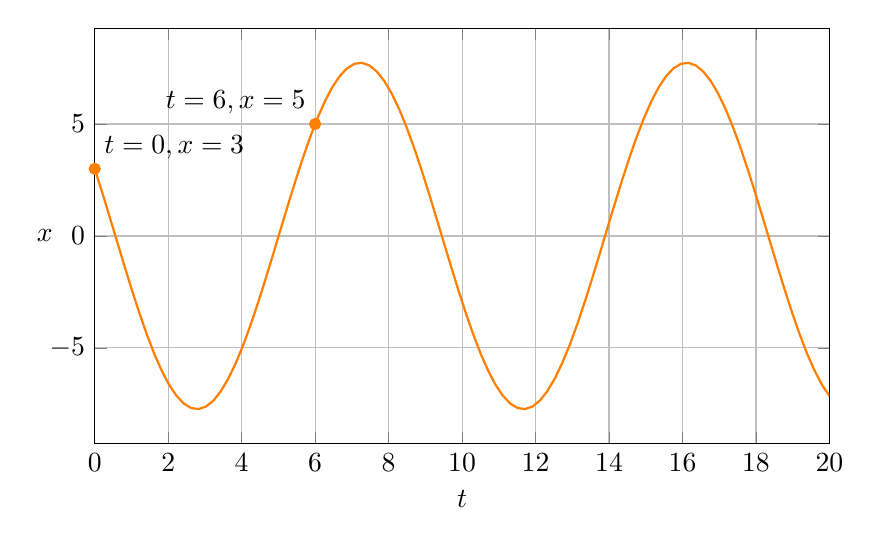
\begin{tikzpicture}
                            \begin{axis}[
                                width=0.9\textwidth, height=2.7in,
                                xmin=0, xmax=20,
                                xlabel={$t$},
                                ylabel={$x$},
                                ylabel shift=-8pt,
                                ylabel style={rotate=-90},
                                grid=major
                            ]
                                \addplot[mark=none, orange, thick, domain=0:20, samples=100] {3*cos(deg(0.707107*x))-7.13033*sin(deg(0.707107*x))};
                                \addplot[mark=*, only marks, orange] coordinates {(0,3) (6,5)};
                                \node at (0,3) [anchor=south west] {$t=0,x=3$};
                                \node at (6,5) [anchor=south east] {$t=6,x=5$};
                            \end{axis}
                        \end{tikzpicture}
                    \end{center}
                }
                \item{
                    \label{part:5d}
                    \textbf{In your own words, describe the motion of the mass with respect to time.}
                    \par
                    The motion is sinusoidal (simple harmonic) with respect to time, with an amplitude of \textasciitilde{}7.74 and a period of \textasciitilde{}8.89. The curve passes through the points $(0,3)$ and $(6,5)$ (indicated on graph), which were my initial conditions.
                }
            \end{enumerate}
            \textbf{\boldmath The above model of a mass on a spring is plausible but not very realistic: in practice, friction will act to decelerate the mass. Including a frictional force with magnitude proportional to velocity (i.e., $\frac{dx}{dt}$), Newton's second law becomes $$m\frac{d^2x}{dt^2}+q\frac{dx}{dt}+kx=0$$ where $q$ is the damping coefficient representing friction.}
            \begin{enumerate}[label={\textbf{(\alph*)}}, resume]
                \item{
                    \textbf{Determine the general solution to this DE using information given in part \ref{part:5a} of this question.}
                    \par
                    According to part \ref{part:5a}, the general solution to a second-order linear differential equation of the form $a\frac{d^2x}{dt^2}+b\frac{dx}{dt}+cx=0$ is given by $$x=e^{rt}(C_1\cos(\omega t)+C_2\sin(\omega t))$$ where $r=-\frac{b}{2a}$ and $\omega=\frac{\sqrt{4ac-b^2}}{2a}$.
                    \par
                    Plugging in $a=m$, $b=q$, and $c=k$ gives $r=-\frac{q}{2m}$ and $\omega=\frac{\sqrt{4mk-q^2}}{2m}$. Putting these into the general solution, we get
                    \begin{equation*}
                        x=e^{-\frac{q}{2m}t}\left(C_1\cos\left(\frac{\sqrt{4mk-q^2}}{2m}t\right)+C_2\sin\left(\frac{\sqrt{4mk-q^2}}{2m}t\right)\right)
                    \end{equation*}
                }
                \item{
                    \textbf{\boldmath Using the same initial conditions and values for $m$ and $k$ from part \ref{part:5c}, set $q=\sqrt{4mk}-1$ (so that $q^2-4mk<0$) and sketch the corresponding solution for values of $t\ge0$.}
                    \par
                    Finding $q$:
                    \begin{align*}
                        q&=\sqrt{4mk}-1 \\
                        &=\sqrt{4(10)(5)}-1 \\
                        &=\sqrt{200}-1
                    \end{align*}
                    Now the solution is
                    \begin{align*}
                        x&=e^{-\frac{\sqrt{200}-1}{2(10)}t}\left(C_1\cos\left(\frac{\sqrt{4(10)(5)-(\sqrt{200}-1)^2}}{2(10)}t\right)+C_2\sin\left(\frac{\sqrt{4(10)(5)-(\sqrt{200}-1)^2}}{2(10)}t\right)\right) \\
                        &=e^{-\frac{\sqrt{200}-1}{20}t}\left(C_1\cos\left(\frac{\sqrt{200-(\sqrt{200}-1)^2}}{20}t\right)+C_2\sin\left(\frac{\sqrt{200-(\sqrt{200}-1)^2}}{20}t\right)\right)
                    \end{align*}
                    which I will approximate as
                    \begin{equation*}
                        x=e^{-0.657107t}(C_1\cos(0.261172t)+C_2\sin(0.261172t))
                    \end{equation*}
                    Recall that my initial values were $$\begin{matrix}t_1=0 & t_2=6 \\ x(t_1)=3 & x(t_2)=5\end{matrix}$$ Using these, I'll solve for $C_1$ and $C_2$.
                    \begin{align*}
                        x(0)=3&=e^{-0.657107(0)}(C_1\cos(0.261172(0))+C_2\sin(0.261172(0))) \\
                        &=e^0(C_1+0) \\
                        C_1&=3
                    \end{align*}
                    \begin{align*}
                        x(6)=5&=e^{-0.657107(6)}(3\cos(0.261172(6))+C_2\sin(0.261172(6))) \\
                        &=0.0193967(0.0112990+C_2\cdot0.999993) \\
                        257.776&=0.0112990+C_2\cdot0.999993 \\
                        C_2\cdot0.999993&=257.765 \\
                        C_2&=257.767
                    \end{align*}
                    The resulting solution is therefore
                    \begin{equation*}
                        x=e^{-0.657107t}(3\cos(0.261172t)+257.767\sin(0.261172t))
                    \end{equation*}
                    \newpage
                    Sketching this solution, I get:
                    \begin{center}
                        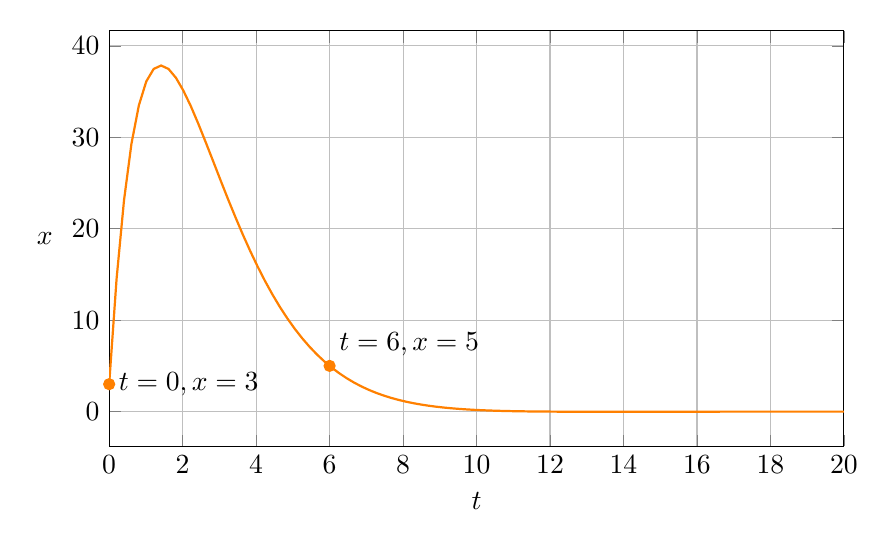
\begin{tikzpicture}
                            \begin{axis}[
                                width=0.9\textwidth, height=2.7in,
                                xmin=0, xmax=20,
                                xlabel={$t$},
                                ylabel={$x$},
                                ylabel style={rotate=-90},
                                grid=major
                            ]
                                \addplot[mark=none, orange, thick, domain=0:20, samples=100] {exp(-0.657107*x)*(3*cos(deg(0.261172*x))+257.767*sin(deg(0.261172*x)))};
                                \addplot[mark=*, only marks, orange] coordinates {(0,3) (6,5)};
                                \node at (0,3) [anchor=west] {$t=0,x=3$};
                                \node at (6,5) [anchor=south west] {$t=6,x=5$};
                            \end{axis}
                        \end{tikzpicture}
                    \end{center}
                }
                \item{
                    \textbf{In your own words, describe the motion of the mass with respect to time. Explain what is different in comparison to what you found when there was no friction (i.e., parts \ref{part:5b}--\ref{part:5d}).}
                    \par
                    The motion has been overdamped. It is still composed of a sinusoidal wave, but now its amplitude decreases exponentially. When there was no friction (part \ref{part:5c}), the motion continued with the same amplitude indefinitely. Now, the motion subsides mostly within ten seconds, although technically the mass never stops moving. Another thing to note is that the curve still passes through the points $(0,3)$ and $(6,5)$, meaning that the solution still satisfies my initial conditions.
                }
            \end{enumerate}
        }
    \end{enumerate}
\end{document}
